\chapter{相互作用}

\section{重力 弹力 摩擦力}


1.重力

(1)产生:由于\_\_地球\_\_的吸引而使物体受到的力.

(2)大小:与物体的质量成\_\_正比\_\_,即$G=m g$.可用\_\_弹簧测力计\_\_测量重力.

(3)方向:总是\_\_竖直向下\_\_的.

(4)重心:其位置与物体的\_\_质量\_\_分布和\_\_形状\_\_有关.

2.弹力

(1)定义:发生\_\_弹性形变\_\_的物体由于要恢复原状而对与它接触的物体产生的作用力.

(2)产生的条件

\ding{172}物体间直接\_\_接触\_\_;\ding{173}接触处发生\_\_弹性形变\_\_.

(3)方向:总是与物体形变的方向\_\_相反\_\_.

3.胡克定律

(1)内容:在\_\_弹性限度\_\_内,弹力的大小跟弹簧伸长(或缩短)的长度x成\_\_正比\_\_.

(2)表达式:$F=kx$.$k$是弹簧的\_\_劲度系数\_\_,由弹簧自身的性质决定,单位是\_\_牛顿每米\_\_,用符号$\mathrm{N} / \mathrm{m}$表示.x是弹簧长度的\_\_变化量\_\_,不是弹簧形变以后的长度.

4.滑动摩擦力和静摩擦力的对比

\begin{longtable}[]{@{}m{2cm}m{6.5cm}m{6.5cm}@{}}
\toprule
名称项目& 
静摩擦力&
滑动摩擦力\tabularnewline
\midrule
\endhead
定义 & 两相对静止的物体间的摩擦力 &
两相对运动的物体间的摩擦力\tabularnewline
产生条件&
\ding{172}接触面粗糙

\ding{173}接触处有压力

\ding{174}两物体间有相对运动趋势
&
\ding{172}接触面粗糙

\ding{173}接触处有压力

\ding{174}两物体间有相对运动
\tabularnewline
大小、方向
& \begin{minipage}[t]{0.30\columnwidth}\raggedright
大小:$0<F_f\le F_{fmax}$

方向:与受力物体相对运动趋势的方向相反\strut
\end{minipage} & \begin{minipage}[t]{0.30\columnwidth}\raggedright
大小:$F_f=\mu F_N$

方向:与受力物体相对运动的方向相反\strut
\end{minipage}\tabularnewline
作用效果 & 总是阻碍物体间的相对运动趋势 &
总是阻碍物体间的相对运动\tabularnewline
\bottomrule
\end{longtable}

滑动摩擦力大小的计算公式$F_{\mathrm{f}}=\mu F_{\mathrm{N}}$中$\mu$为比例常数,称为动摩擦因数,其大小与两个物体的材料和接触面的粗糙程度有关.

\newpage
\subsection{弹力有无的判断}

\begin{longtable}[]{@{}m{1cm}m{6.1cm}m{2cm}m{4cm}@{}}
	\toprule
	方法& 概念& 图示&说明 \tabularnewline
	\midrule
	假
	
	设
	
	法& 假设将与研究对象接触的物体解除接触,判断研究对象的运动状态是否发生改变,若运动状态不变,则此处不存在弹力,若运动状态改变,则此处一定存在弹力  &
	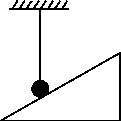
\includegraphics[height=0.55208in]{media/image40.png}&
	图中细线竖直、斜面光滑,因去掉斜面体,小球的状态不变,故小球只受细线的拉力,不受斜面的支持力\tabularnewline
	
	替
	
	换
	
	法 & 用细绳替换装置中的杆件,看能不能维持原来的力学状态,如果能维持,则说明这个杆提供的是拉力;否则,提供的是支持力&
	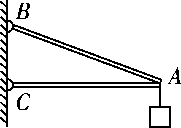
\includegraphics[height=0.48333in]{media/image41.png}&
	图中轻杆AB、AC,用绳替换AB,原装置状态不变,说明AB对A施加的是拉力;用绳替换AC,原状态不能维持,说明AC对A施加的是支持力\strut
	\tabularnewline
	状
	
	态
	
	法 & 由运动状态分析弹力,即物体的受力必须与物体的运动状态相符合,依据物体的运动状态,由二力平衡(或牛顿第二定律)列方程,求解物体间的弹力 &
	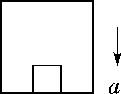
\includegraphics[height=0.42708in]{media/image42.png}&
	升降机以a=g加速下降时物体不受底板的弹力作用\tabularnewline
	\bottomrule
	\end{longtable}
{[}例1{]}(2017·陕西西安调研)如图所示,在一个正方体的盒子中放有一个质量分布均匀的小球,小球的直径恰好和盒子内表面正方体的棱长相等,盒子沿倾角为$\alpha$的固定斜面滑动,不计一切摩擦,下列说法中正确的是( A )

\begin{center}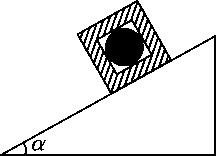
\includegraphics[width=0.97917in,height=0.70833in]{media/image43.png}\end{center}

A.无论盒子沿斜面上滑还是下滑,球都仅对盒子的下底面有压力

B.盒子沿斜面下滑时,球对盒子的下底面和右侧面有压力

C.盒子沿斜面下滑时,球对盒子的下底面和左侧面有压力

D.盒子沿斜面上滑时,球对盒子的下底面和左侧面有压力

{[}思维导引{]}采用假设法,可假设小球仅对盒子的下底有压力,判断两者运动是否相同.
\begin{solution}
	先以盒子和小球组成的系统为研究对象,无论上滑还是下滑,用牛顿第二定律均可求得系统的加速度大小为a=gsin
$\alpha$,方向沿斜面向下,由于盒子和小球始终保持相对静止,所以小球的加速度大小也是a=gsin
$\alpha$,方向沿斜面向下,小球沿斜面向下的重力分力大小恰好等于所需的合外力,因此不需要盒子的左、右侧面提供弹力.故选项A正确.
\end{solution}

\begin{center}
\includegraphics[width=0.70833in,height=0.125in]{media/image44.png}\end{center}
对于形变明显的物体,由形变情况直接判断弹力情况,对于形变不明显的物体通常用``假设法''和``替换法'',有时要根据物体的运动状态判定弹力情况.

\subsection{弹力方向的确定和大小的计算}

1.弹力方向的确定

\begin{center}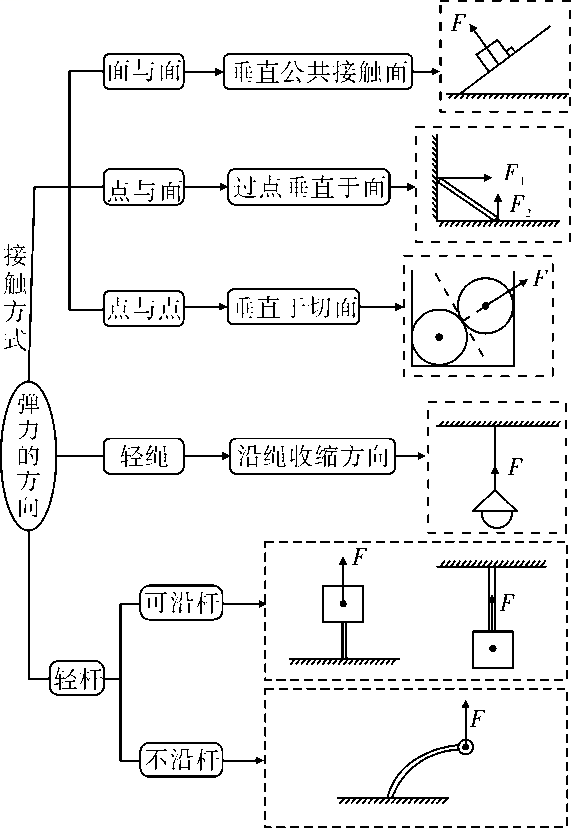
\includegraphics[width=2in]{media/image45.png}\end{center}
2.计算弹力大小的三种方法

(1)根据胡克定律进行求解.(2)根据力的平衡条件进行求解.(3)根据牛顿第二定律进行求解.

{[}例2{]}如图所示,固定在小车支架上的斜杆与竖直杆的夹角为$\theta$,在斜杆下端固定一个质量为m的小球,下列关于杆对球的作用力F的判断中正确的是( D )\begin{center}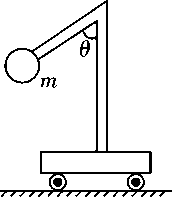
\includegraphics[width=0.78125in,height=0.89583in]{media/image46.png}\end{center}

A.小车静止时,$F=mg\cos \theta$,方向沿杆向上

B.小车静止时,$F=mg\cos \theta$,方向垂直杆向上

C.小车向右以加速度a运动时,一定有$F=\dfrac{mg}{\sin\theta}$

D.小车向左以加速度a运动时,$F=\sqrt{(ma)^2+(mg)^2}$,方向斜向左上方,与竖直方向的夹角为$\alpha$满足$tan\alpha=\dfrac{a}{g}$

{[}例3{]}缓冲装置可抽象成如图所示的简单模型,图中A、B为原长相等、劲度系数分别为$k_1$、$k_2$($k_1\neq k_2$)的两个不同的轻质弹簧.下列表述正确的是( D )

\begin{center}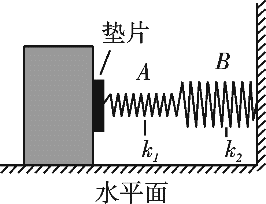
\includegraphics[width=1.20833in,height=0.92708in]{media/image47.png}\end{center}

A.装置的缓冲效果与两弹簧的劲度系数无关

B.垫片向右移动稳定后,两弹簧产生的弹力之比$F_1:F_2=k_1:k_2 $

C.垫片向右移动稳定后,两弹簧的长度之比$l_1:l_2=k_2:k_1$

D.垫片向右移动稳定后,两弹簧的压缩量之比$x_1:x_2=k_2:k_1$ 

{[}思维导引{]}\ding{172}分析稳定后,两弹簧之间相互弹力作用的关系.\ding{173}利用胡克定律计算两个弹簧的形变量和长度.

\subsection{静摩擦力的大小和方向}

1.静摩擦力有无的判断

(1)假设法

静摩擦力的方向一定与物体相对运动趋势的方向相反,利用``假设法''可以判断出物体相对运动趋势的方向.

假设法(如图所示)

\begin{center}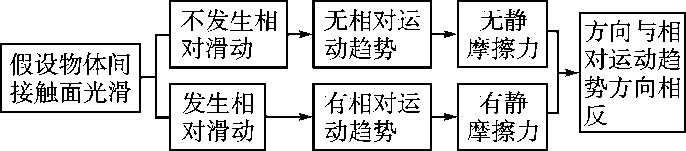
\includegraphics[width=3.11458in,height=0.6875in]{media/image48.png}\end{center}

(2)状态法

此法关键是先判明物体的运动状态(即加速度的方向),再利用牛顿第二定律(F=ma)确定合力,然后通过受力分析确定静摩擦力的大小及方向.

(3)牛顿第三定律法

此法的关键是抓住``力是物体间的相互作用'',先确定受力较少的物体受到的静摩擦力的方向,再根据``力的相互性''确定另一物体受到的静摩擦力方向.

2.静摩擦力的计算方法

(1)最大静摩擦力$F_{fmax}$的计算

最大静摩擦力$F_{fmax}$只在刚好要发生相对滑动这一特定状态下才表现出来.比滑动摩擦力稍大些,通常认为二者相等,即$F_{fmax}=\mu F_N$. 

(2)一般静摩擦力的计算

一般静摩擦力F的大小和方向都与产生相对运动趋势的力密切相关,跟接触面间相互挤压的弹力$F_N$无直接关系,因此具有大小、方向的可变性.对具体问题要结合研究对象的运动状态(静止、匀速运动或加速运动),利用平衡条件或牛顿运动定律列方程求解.



\begin{center}
\includegraphics[width=0.70833in,height=0.125in]{media/image34.png}\end{center}
\begin{center}
	\textbf{应用"状态法"解题时应注意的问题}
\end{center}

状态法是分析判断静摩擦力有无及方向、大小的常用方法,在使用状态法处理问题时,需注意以下两点:

(1)明确物体的运动状态,分析物体的受力情况,根据平衡方程或牛顿定律求解静摩擦力的大小和方向.

(2)静摩擦力的方向与物体的运动方向没有必然关系,可能相同,也可能相反,还可能成一定的夹角.
\newpage
\subsection{滑动摩擦力的大小和方向}

1.产生的条件

(1)两物体相互接触且挤压,发生形变,产生弹力.

(2)两接触面粗糙.

(3)两物体沿接触面发生相对运动.

以上三个条件必须同时具备,才会有滑动摩擦力存在.

2.在计算滑动摩擦力的公式$F_f=\mu F_N$中,$\mu$为动摩擦因数,其大小与接触面的材料、表面的粗糙程度有关;$F_N$为两接触面间的正压力,其大小不一定等于物体的重力.

3.滑动摩擦力的大小与物体的运动速度无关,与接触面积也无关.

4.滑动摩擦力的方向总是与物体间相对运动的方向相反,但不一定与物体运动方向相反.

{[}例5{]}(2017·吉林长春检测)如图所示,质量为m的工件置于水平放置的钢板C上,二者间动摩擦因数为$\mu$,由于固定的光滑导槽A、B的控制,工件只能沿水平导槽运动,现使钢板以速度$v_1$向右运动,同时用F拉动工件(F方向与导槽平行)使其以速度$v_2$沿导槽运动,则F的大小为( C )

\begin{center}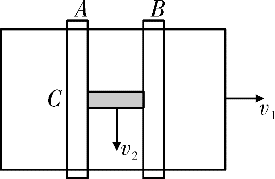
\includegraphics[width=1.25in,height=0.8125in]{media/image50.png}\end{center}

A.等于$\mu mg$ B.大于$\mu mg$

C.小于$\mu mg$ D.不能确定
\begin{solution}
	钢板以速度$v_1$向右运动,则工件以等大速度相对钢板向左移动,设为$v_1^{\prime}$,同时工件被拉动也具有另一速度$v_2$,故工件相对于钢板的运动速度应是$v_1^{\prime}$与$v_2$的合成,即如上图中的速度v.滑动摩擦力阻碍二者的相对运动,故工件所受摩擦力$F_f$与v方向相反,要使工件沿导槽匀速运动,所施加的拉力只需与$F_f$一个分力平衡,故 $F< F_f=\mu mg$.
\end{solution}

\begin{center}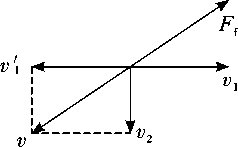
\includegraphics[width=1.08333in,height=0.66667in]{media/image51.png}\end{center}
\newpage
\subsection{摩擦力突变问题}

\begin{center}
\includegraphics[width=0.70833in,height=0.125in]{media/image37.png}\end{center}
\begin{center}
	\textbf{解决摩擦力突变问题的关键点}
\end{center}

物体受到的外力发生变化时,物体受到的摩擦力的种类就有可能发生突变.解决这类问题的关键是:正确对物体受力分析和运动状态分析,从而找到物体摩擦力的突变``临界点''.

常见类型如下:

(1)静---静``突变''

当作用在物体上的其他力的合力发生变化时,物体仍保持静止,而所受静摩擦力方向发生$180^\circ$``突变'',则``突变''点是静摩擦力为零时.

(2)动---动``突变''

某物体相对于另一物体滑动的过程中,若相对运动方向变了,则滑动摩擦力方向发生``突变'',``突变''点为两物体相对速度为零时.

(3)静---动``突变''

物体在摩擦力和其他力作用下处于静止状态,当其他力变化时,如果物体不能保持静止状态,则物体受到的静摩擦力将``突变''成滑动摩擦力,``突变''点为静摩擦力达到最大值时.

(4)动---静``突变''

两物体相对减速滑动的过程中,若相对速度变为零,则滑动摩擦力``突变''为静摩擦力,``突变''点为两物体相对速度刚好为零时.

{[}例6{]}(多选)如图所示,将两相同的木块a、b置于粗糙的水平地面上,中间用一轻弹簧连接,两侧用细绳系于墙壁.开始时a、b均静止,弹簧处于伸长状态,两细绳均有拉力,a所受摩擦力$F_{fa}\neq 0$,b所受摩擦力$F_{fb}=0$.现将右侧细绳剪断,则剪断瞬间( AD )

\begin{center}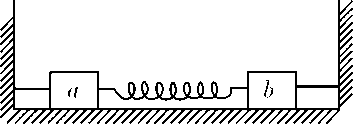
\includegraphics[width=1.60417in,height=0.5625in]{media/image52.png}\end{center}

A.$F_{fa}$大小不变 B.$F_{fa}$方向改变
C.$F_{fb}$仍然为零 D.$F_{fb}$方向向右

{[}例7{]}传送带以恒定的速率v=10m/s运动,已知它与水平面成$\alpha=37^\circ$,如图所示,PQ=16m,将一个小物体无初速度地放在P点,小物体与传送带间的动摩擦因数为$\mu=0.5$,问当传送带逆时针转动时,小物体运动到Q点的时间为多少?($cos37^\circ=0.8,sin 37^\circ=0.6$,g取$10 m/s^2$)

\begin{center}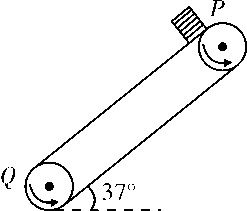
\includegraphics[width=1.125in,height=0.95833in]{media/image53.png}\end{center}

\begin{solution}
	2 s
\end{solution}
\begin{center}
\includegraphics[width=0.70833in,height=0.125in]{media/image25.png}\end{center}
\begin{center}
	\textbf{摩擦力突变问题的分析步骤}
\end{center}

\begin{center}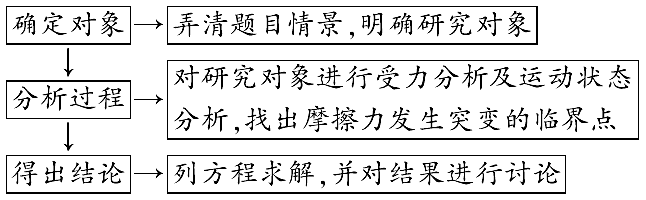
\includegraphics[width=2.8125in,height=0.875in]{media/image54.png}\end{center}

\newpage
\section{力的合成与分解}

1.力的合成

(1)合力与分力

\ding{172}定义:如果几个力共同作用产生的效果与一个力的作用效果相同,这一个力就叫做那几个力的\_\_合力\_\_,那几个力叫做这一个力的\_\_分力\_\_.

\ding{173}关系:合力与分力是\_\_等效替代\_\_关系.

(2)共点力

作用在物体的\_\_同一点\_\_,或作用线的\_\_延长线\_\_交于一点的几个力.

\begin{center}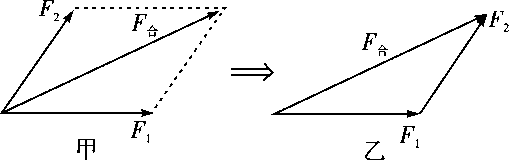
\includegraphics[width=2.3125in,height=0.72917in]{media/image61.png}\end{center}
(3)力的合成

\ding{172}定义:求几个力的\_\_合力\_\_的过程.

\ding{173}运算法则

平行四边形定则:求两个互成角度的\_\_共点力\_\_的合力,可以用表示这两个力的线段为邻边作平行四边形,这两个邻边之间的对角线就表示合力的\_\_大小\_\_和\_\_方向\_\_(图甲).

三角形定则:把两个矢量的首尾顺次连接起来,第一个矢量的首到第二个矢量的尾的\_\_有向线段\_\_为合矢量(图乙).

2.力的分解

(1)定义

求一个力的\_\_分力\_\_的过程,力的分解是\_\_力的合成\_\_的逆运算.

(2)遵循的原则

\ding{172}\_\_平行四边形\_\_定则.

\ding{173}\_\_三角形\_\_定则.

(3)分解方法

\ding{172}力的作用效果分解法.

\ding{173}正交分解法.

3.矢量和标量

(1)矢量

既有大小又有\_\_方向\_\_的物理量,相加时遵循\_\_平行四边形\_\_定则.如速度、力等.

(2)标量

只有大小没有\_\_方向\_\_的物理量,求和时按算术法则相加.如路程、动能等.
\newpage
\subsection{共点力的合成}

1.共点力合成的常用方法

(1)作图法

从力的作用点沿两个分力的作用方向按同一标度作出两个分力$F_1$、$F_2$,以这两个力为邻边作一个平行四边形,这两个力所夹对角线表示这两个力的合力.通常可分别用刻度尺和量角器直接量出合力的大小和方向.

(2)解析法

根据力的平行四边形定则作出力的合成的图示,如图所示.

\begin{center}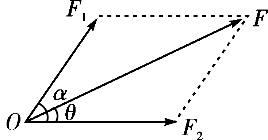
\includegraphics[width=1.21875in,height=0.63542in]{media/image64.png}\end{center}

$F=\sqrt{F_1^2+F_2^2+2F_1F_2\cos\alpha}$.

它与$F_2$的夹角为$\theta$,$\tan \theta=\dfrac{F_1\sin\alpha}{F_2+F_1\cos\alpha}$.

2.几种特殊情况的共点力的合成

\begin{longtable}[]{@{}m{4cm}m{3cm}m{3cm}@{}}
\toprule
类型 & 作图 & 合力的计算\tabularnewline
\midrule
\endhead

互相垂直& \begin{center}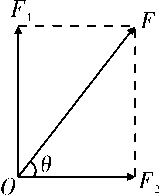
\includegraphics[width=0.5in]{media/image65.png}\end{center}&
$F=\sqrt{F_1^2+F_2^2}$

$\tan\theta=\dfrac{F_1}{F_2}$\tabularnewline

两力等大,夹角$\theta$ &
\begin{center}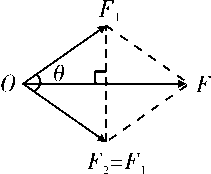
\includegraphics[width=0.7in,]{media/image66.png}\end{center}
&
$F=2F_1\cos\dfrac{\theta}{2}$

$F$与$F_1$夹角为$\dfrac{\theta}{2}$\tabularnewline
两力等大且夹角$120^\circ$ &
\begin{center}
	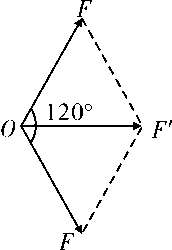
\includegraphics[width=0.6in]{media/image67.png}
\end{center}
 &
合力与分力等大\tabularnewline
\bottomrule
\end{longtable}

\begin{center}
\includegraphics[width=0.70833in,height=0.125in]{media/image34.png}\end{center}
\begin{center}
	\textbf{作图法求合力的四点要求}
\end{center}

(1)分力、合力的作用点相同,切忌弄错表示合力的对角线

(2)分力、合力的比例要一致,力的标度要适当

(3)虚线、实线要分清,表示分力和合力的两条邻边和对角线画成实线,并加上箭头,平行四边形的另两条边画成虚线

(4)求合力时既要求出合力的大小,又要求出合力的方向

{[}例1{]}(2017·天津卷)(多选)如图所示,轻质不可伸长的晾衣绳两端分别固定在竖直杆M、N上的a、b两点,悬挂衣服的衣架挂钩是光滑的,挂于绳上处于静止状态.如果只人为改变一个条件,当衣架静止时,下列说法正确的是( AB )

\begin{center}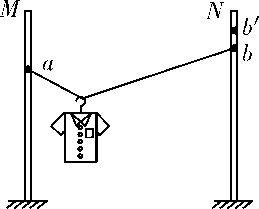
\includegraphics[width=1.17708in,height=0.94792in]{media/image68.png}\end{center}

A.绳的右端上移到$b^{\prime}$,绳子拉力不变

B.将杆N向右移一些,绳子拉力变大

C.绳的两端高度差越小,绳子拉力越小

D.若换挂质量更大的衣服,则衣架悬挂点右移
\begin{solution}
	oa、ob为一根绳,两端拉力相等,设绳aob长为L,M、N的水平距离为d,bo延长线交M于$a^{\prime}$,由几何知识知$a^{\prime}o=ao$,$\sin\theta=\dfrac{d}{L}$,由平衡条件有$2F\cos\theta=mg$,则$F=\dfrac{mg}{2\cos\theta^{\prime}}$,当b上移到$b^{\prime}$时,d、L不变,$\theta$不变,故F不变,选项A正确,C错误.将杆N向右移一些,L不变,d变大,$\theta$变大,$\cos\theta$变小,则F变大,选项B正确.只改变m,其他条件不变,则$\sin\theta$不变,$\theta$不变,衣架悬挂点不变,选项D错误.
\end{solution}


\begin{center}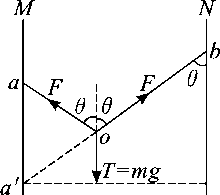
\includegraphics[width=1in,height=0.88542in]{media/image69.png}\end{center}
\begin{center}
\includegraphics[width=0.70833in,height=0.125in]{media/image13.png}\end{center}

(1)力合成时,要正确理解合力与分力的大小关系:合力与分力的大小关系要视情况而定,不能形成合力总大于分力的思维定式.

(2)合力与它的分力是等效替代关系,在进行有关力的计算时,如果已计入了合力,就不能再计入分力;如果已计入了分力,就不能再计入合力.
\newpage
\subsection{力的分解}

1.按力的作用效果分解(思路图)

\begin{center}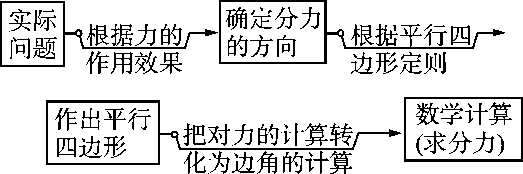
\includegraphics[width=2.375in,height=0.79167in]{media/image70.png}\end{center}

如图所示,物体的重力G按产生的效果分解为两个分力,$F_1$使物体下滑,$F_2$使物体压紧斜面.

\begin{center}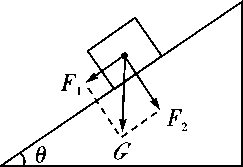
\includegraphics[width=1.10417in,height=0.76042in]{media/image71.png}\end{center}

2.正交分解法

(1)定义:将已知力按互相垂直的两个方向进行分解的方法.

(2)建立坐标轴的原则:一般选共点力的作用点为原点,在静力学中,以少分解力和容易分解力为原则(使尽量多的力在坐标轴上);在动力学中,往往以加速度方向和垂直加速度方向为坐标轴建立坐标系.

(3)方法:物体受到多个力$F_1$、$F_2$、$F_3$\ldots\ldots 作用,求合力F时,可把各力向相互垂直的x轴、y轴分解.

\begin{center}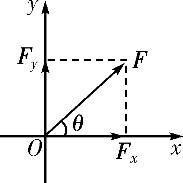
\includegraphics[width=0.83333in,height=0.83333in]{media/image72.png}\end{center}

x轴上的合力:

$F_x=F_{x1}+F_{x2}+F_{x3}+\ldots\ldots{}$

y轴上的合力:

$F_y=F_{y1}+F_{y2}+F_{y3}+\ldots\ldots{}$

合力大小:

$F=\sqrt{F_x^2+F_y^2}$

合力方向:与x轴夹角为$\theta$,则$\tan \theta=\dfrac{F_y}{F_x}$.

{[}例2{]}如图所示,光滑斜面的倾角为$\theta$,有两个相同的小球,分别用光滑挡板A、B挡住,挡板A沿竖直方向,挡板B垂直于斜面,则两挡板受到小球压力的大小之比为\_\_$1:\cos\theta$\_\_,斜面受到两个小球压力大小之比为\_\_$1:\cos^2\theta$\_\_.

\begin{center}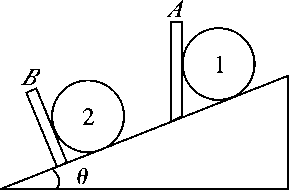
\includegraphics[width=1.3125in,height=0.86458in]{media/image73.png}\end{center}

{[}思维导引{]}既然求解的是挡板和斜面实际受到的压力,就应按力的作用效果分解力.

\subsection{``绳------杆''模型}

1.``死结''与``活结''模型

(1)``死结''可理解为把绳子分成两段,且不可以沿绳子移动的结点.``死结''两侧的绳因结而变成了两根独立的绳.

(2)``活结''可理解为把绳子分成两段,且可以沿绳子移动的结点.``活结''一般是由绳跨过滑轮或者绳上挂一光滑挂钩而形成的.实质还是同一根绳子.

2.``固定杆''与``活动杆''模型

(1)一般情况下,插入墙中的杆属于固定杆(如钉子).

(2)一端用铰链相连的杆属于活动杆.

\begin{center}
\includegraphics[width=0.70833in,height=0.125in]{media/image37.png}\end{center}

\begin{center}
	\textbf{"绳杆"模型的处理方法}
\end{center}

(1)无论``死结''还是``活结''一般均以结点为研究对象进行受力分析.

(2)由``死结''分开的两段绳子上的弹力不一定相等;由``活结''分开的两段绳子上弹力的大小一定相等,两段绳子合力的方向一定沿这两段绳子夹角的平分线.

(3)固定杆的弹力方向不一定沿杆的方向,而活动杆的弹力方向一定沿杆的方向.

{[}例3{]}如图甲所示,细绳AD跨过固定的水平轻杆BC右端的定滑轮挂住一个质量为$M_1$的物体,$\angle ACB=30^\circ$;图乙中轻杆HG一端用铰链固定在竖直墙上,另一端G通过细绳EG拉住,EG与水平方向也成$30^\circ$,轻杆的G点用细绳GF拉住一个质量为$M_2$的物体.求:

\begin{center}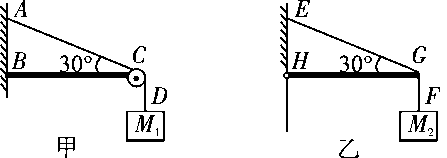
\includegraphics[width=2.03125in,height=0.71875in]{media/image74.png}\end{center}

(1)细绳AC段的张力$F_{AC}$与细绳EG的张力$F_{EG}$之比;

(2)轻杆BC对C端的支持力;

(3)轻杆HG对G端的支持力.

{[}思维导引{]}(1)判断杆的作用力方向是否沿杆方向.(2)选取恰当的研究对象.
\begin{solution}

	(1)$\dfrac{M_1}{2M_2}$ 
	
	(2)$M_1g$,方向与水平方向成$30^\circ$指向右上方
	
	(3)$\sqrt{3} M_2g$,方向水平向右
\end{solution}


\newpage
\section{受力分析 共点力的平衡}


1.受力分析

(1)定义

把指定物体(研究对象)在特定的物理环境中受到的所有外力都找出来,并画出受力图,这个过程就是受力分析.

(2)受力分析的顺序

先找重力,再找接触力(弹力、摩擦力),最后分析电场力、磁场力及其他力.

(3)受力分析的步骤

\ding{172}明确研究对象------确定分析受力的物体,研究对象可以是单个物体,也可以是多个物体的组合.

\ding{173}隔离物体分析------将研究对象从周围物体中\_\_隔离\_\_出来,进而分析物体受的重力、弹力、摩擦力、电磁力等,检查周围有哪些物体对它施加了力的作用.

\ding{174}画出受力示意图------边分析边将力一一画在受力示意图上,准确标出\_\_方向\_\_.

\ding{175}检查画出的每一个力能否找出它的\_\_施力物体\_\_,检查分析结果能否使研究对象处于题目所给的运动状态,否则,必然发生了漏力、添力或错力现象.

2.共点力的平衡

(1)平衡状态:物体处于静止或\_\_匀速直线运动\_\_状态.

(2)共点力的平衡条件:$F_{\text{合}}=0$或者$\left\{\begin{array}{l}F_{x}=0 \\ F_{y}=0\end{array}\right.$

(3)平衡条件的推论.

\ding{172}二力平衡

如果物体在两个共点力的作用下处于平衡状态,这两个力必定大小\_\_相等\_\_、方向\_\_相反\_\_,为一对平衡力.

\ding{173}三力平衡

如果物体在三个共点力的作用下处于平衡状态,其中任意两个力的合力一定与第三个力大小\_\_相等\_\_、方向\_\_相反\_\_.

\ding{174}多力平衡

如果物体受多个力作用处于平衡状态,其中任何一个力与其余力的合力大小\_\_相等\_\_、方向\_\_相反\_\_.

{[}思考感悟{]}(1)物体在某一时刻速度为零时,物体不一定处于平衡状态.(2)在多个共点力作用下的物体处于静止状态,如果其中一个力消失其他力保持不变,物体沿消失的力的反方向做初速度为零的匀加速直线运动.
\newpage
\subsection{物体的受力分析}

\begin{center}
\includegraphics[width=0.70833in,height=0.125in]{media/image37.png}\end{center}
\begin{center}
	\textbf{整体法,隔离法在受力分析时的灵活运用}
\end{center}

(1)当所涉及的物理问题是整体与外界作用时,应用整体分析法,可使问题简单明了,而不必考虑内力的作用.

(2)当涉及的物理问题是物体间的相互作用时,应用隔离分析法,这时系统中物体间相互作用的内力就会变为各个独立物体的外力.

{[}例1{]}(2018·浙江宁波调研)如图所示,斜面小车M静止在光滑水平面上,一边紧贴墙壁.若再在斜面上加一物体m,且M、m相对静止,小车后来受力个数为( B )

\begin{center}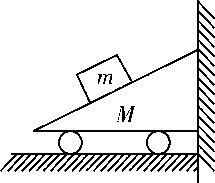
\includegraphics[width=0.97917in,height=0.83333in]{media/image82.png}\end{center}

A.3 

B.4

C.5 

D.6
\begin{solution}
	对M和m整体,它们必受到重力和地面支持力,因小车静止,由平衡条件知墙面对小车必无作用力.以小车为研究对象,如右图所示,它受四个力:重力Mg,地面的支持力$F_{N1}$,m对它的压力$F_{N2}$和摩擦力$F_f$.由于m静止,可知$F_f$和$F_{N2}$的合力必竖直向下,故选项B正确.
\end{solution}

\begin{center}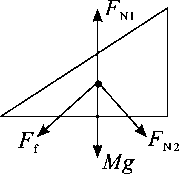
\includegraphics[width=0.8125in,height=0.79167in]{media/image83.png}\end{center}
\newpage
\subsection{解决平衡问题常用的方法}

\begin{longtable}[]{@{}m{2.5cm}m{10.5cm}@{}}
\toprule
方法 & 内容\tabularnewline
\midrule
\endhead
分解法 &
物体受到几个力的作用,将某一个力按力的效果进行分解,则其分力和其他力在所分解的方向上满足平衡条件\tabularnewline
合成法 &
物体受几个力的作用,通过合成的方法将它们简化成两个力,这两个力满足二力平衡条件\tabularnewline
正交分解法 &
将处于平衡状态的物体所受的力分解为相互正交的两组,每一组的力都满足二力平衡条件\tabularnewline
力的三角形法 &
物体受同一平面内三个互不平行的力的作用平衡时,这三个力的矢量箭头首尾相接,构成一个矢量三角形;反之,若三个力矢量箭头首尾相接恰好构成三角形,则这三个力的合力必为零.利用三角形法,根据正弦定理、余弦定理或相似三角形等数学知识可求得未知力\tabularnewline
\bottomrule
\end{longtable}

{[}例2{]}(2018·湖南常德模拟)如图所示,重为G的均匀链条,两端用等长的轻绳连接,挂在等高的地方,轻绳与水平方向成$\theta$角.试求:

\begin{center}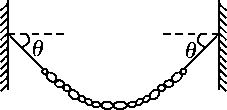
\includegraphics[width=1.03125in,height=0.5in]{media/image84.png}\end{center}

(1)绳子的拉力;

(2)链条在最低点的相互拉力的大小.
\begin{solution}
	(1)$\dfrac{G}{2\sin\theta}$ (2)$\dfrac{1}{2} G\cot \theta$
\end{solution}

\begin{center}
\includegraphics[width=0.70833in,height=0.125in]{media/image13.png}


\end{center}
\begin{center}
	\textbf{应用平衡条件解题步骤}
\end{center}

(1)选取研究对象:根据题目要求,选取一个平衡体(单个物体或系统,也可以是结点)作为研究对象.

(2)画受力示意图:对研究对象进行受力分析,画出受力示意图.

(3)三个力直接合成或正交分解,四个及四个以上的力正交分解.

(4)列方程求解:根据平衡条件列出平衡方程,解平衡方程,对结果进行讨论.
\newpage
\subsection{动态平衡问题}

1.动态平衡

在某一物理过程中,物体或系统始终处于平衡状态,而物体或系统受到的力有一部分是变力(力的大小变或方向变或大小和方向均发生变化),这样的物理过程叫动态平衡.

2.基本思路

化``动''为``静'',``静''中求``动''.

3.``两种''典型方法

\begin{center}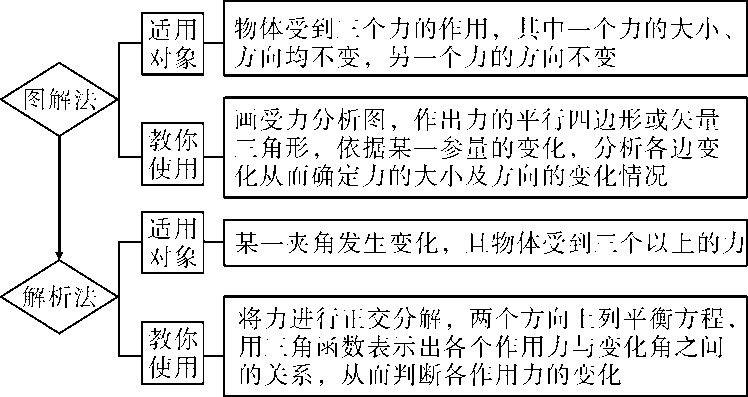
\includegraphics[width=3.39583in,height=1.80208in]{media/image85.png}\end{center}

{[}例3{]}(2017·江苏南京调研)(多选)如图所示,在粗糙水平地面上放着一个截面为四分之一圆弧的柱状物体A,A的左端紧靠竖直墙,A与竖直墙之间放一光滑圆球B,已知A的圆半径为球B的半径的3倍,球B所受的重力为G,整个装置处于静止状态.设墙壁对B的压力为$F_1$,A对B的压力为$F_2$,则若把A向右移动少许后,它们仍处于静止状态,则$F_1$、$F_2$的变化情况分别是( AD )

\begin{center}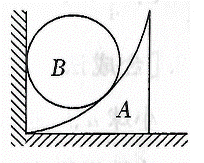
\includegraphics[width=0.92708in,height=0.73958in]{media/image86.png}\end{center}

A.$F_1$减小 

B.$F_1$增大

C.$F_2$增大 

D.$F_2$减小
\newpage
\subsection{平衡中的临界与极值问题}

1.临界问题

当某物理量变化时,会引起其他几个物理量的变化,从而使物体所处的平衡状态``恰好出现''或``恰好不出现'',在问题的描述中常用``刚好''\,``刚能''\,``恰好''等语言叙述.

2.极值问题

平衡物体的极值,一般指在力的变化过程中的最大值和最小值问题.

3.解决平衡中临界与极值问题的常用方法

(1)图解法:根据物体的平衡条件,作出力的矢量图,通过对物理过程的分析,利用平行四边形定则进行动态分析,确定最大值与最小值.

(2)数学解法:通过对问题的分析,依据物体的平衡条件写出物理量之间的函数关系(或画出函数图象),用数学方法求极值(如求二次函数极值、公式极值、三角函数极值).

{[}例4{]}(2018·云南师大附中质检)如图所示,质量为m的小球与细线连接且静止于光滑斜面上,斜面足够长,倾角$\alpha=30^\circ$的斜面体置于光滑水平面上,用水平力F推斜面体使斜面体缓慢地向左移动,小球沿斜面缓慢升高.当细线拉力最小时,推力F等于( A )

\begin{center}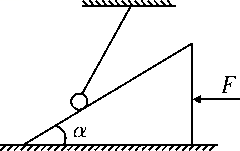
\includegraphics[width=1.09375in,height=0.6875in]{media/image87.png}\end{center}

A.$\dfrac{\sqrt{3}}{4} mg$ 

B.$\dfrac{\sqrt{3}}{2} mg$

C.mg 

D.$\sqrt{3} mg$
\begin{solution}
	小球受力动态平衡如图,可知当$T$平行于斜面时$T_{min}=mg\sin 30^\circ$,对小球和斜面体组成的系统,$F=T_{min}\cos 30^\circ=mg$,选项A正确.
	\begin{center}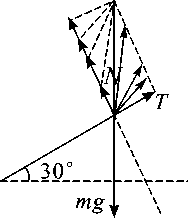
\includegraphics[height=0.98958in]{media/image88.png}\end{center}
\end{solution}
